\chapter{Álgebra vectorial}


\setcounter{section}{1}
\section{El espacio vectorial de las n-plas de números reales}

%--------------------definición 12.1.
\begin{tcolorbox}[colframe = white]
    \begin{def.} Dos vectores $A$ y $B$ de $V_n$ son iguales siempre que coinciden sus componentes. Esto es, si $A=(a_1,a_2,...,a_n)$ y $B=(b_1,b_2,...,b_3)$, la ecuación vectorial $A=B$ tiene exactamente el mismo significado que las $n$ ecuaciones escalares $$a_1=b_1, \qquad a_2=b_2, \qquad a_n=b_n$$
    La suma $A+B$ se define como el vector obtenido sumando los componentes correspondientes: $$A+B = (a_1+b_1,a_2+b_2,...,a_n+b_n)$$
    La $c$ es un escalar, definimos $cA$ o $Ac$ como el vector obtenido multiplicando cada componente de $A$ por $c$: $$cA=(ca_1,ca_2,...,ca_n)$$
    \end{def.}
\end{tcolorbox}

%--------------------teorema 12.1
\begin{teo}

\begin{enumerate}[\bfseries a.]
    \item La adición de vectores es conmutativa. $$A+B=B+A$$\\
	Demostración.-\; Sea $V_n$ el espacio vectorial n-plas y $A=(a_1,a_2,...,a_n)$ y $B=(b_1,b_2,...b_n)$, por lo tanto por definición de adición  y propiedad de números reales, tenemos $$A+B = (a_1+b_1,a_2+b_2,...,a_n+b_n) = (b_1+a_1,b_2+a_2,...,b_n+a_n) = B+A$$.\\

    \item y asociativa, $$A+(B+C) = (A+B)+C$$\\
	Demostración.-\; Sea $V_n$ el espacio vectorial n-plas y $A = (a_1,a_2,...,a_n)$, $B=(b_1,b_2,...,b_n)$ y $C=(c_1,c_2,...,c_n)$ entonces $$A+(B+C) = A + (b_1+c_1,b_2+c_2,...,b_n+c_n) = (a_1+(b_1+c_1),a_2+(b_2+c_2),...,a_1+(b_n+c_n)) = $$
	$$((a_1+b_1)+c_1,(a_2+b_2)+c_2,...,(a_n+b_n)+c_n) = (a_1+b_1,a_2+b_2,...,b_n+c_n)+C = (A+B)+C$$\\

    \item La multiplicación por escalares es asociativa $$c(dA)=(cd)A$$\\
	Demostración.-\; Sea $c,d \in \mathbb{R}$ y $A\in V_n$ entonces 
	\begin{center}
	    \begin{tabular}{rcl}
		$c(dA)$&$=$&$c(da_1,da_2,...,da_n)$\\
		&$=$&$((cd)a_1,(cd)a_2,...,(cd)a_3)$\\
		&$=$&$(cd)A$\\\\
	    \end{tabular}
	\end{center}

    \item y satisface las dos leyes distributivas $$c(A+B)=cA+cB,\quad y \quad (c+d)A=cA+dA$$\\
	Demostración.-\; Las demostraciones son fáciles de realizar siempre y cuando se tomen en cuenta Las definiciones de 12.1.\\\\

    \item El vector con todos los componentes $0$ se llama vector cero y se representa con $O$. Tiene la propiedad.\\\\
	Demostración.-\; Existencia. Sea $O = (o,o,...,o)$ de donde $A+O = (a_1,a_2,...,a_n)+(o,o,...,o) = (a_1+o,a_2+o,...,a_n+o) = (a_1,a_2,...,a_n) = A$.\\
	Unicidad. Supongamos que $O,O^{'} \in V_n; O\neq O$ tal que 
	$$\left\{ \begin{array}{ccc} A+O=A&tomando \; A=O^{'}:&O^{'}+O = O^{'}\\ A+O^{'} = A&tomando \; A=O:&O+O^{'}=O\\ \end{array} \right.$$
	Por lo tanto $O=O^{'}$.\\\\
    \item El vector $(-1)A$ que también se representa con $-A$ se llama el apuesto a $A$. También escribimos $A-B$ en lugar de $A+(-B)$ y lo llamamos diferencia de $A$ y $B$. La ecuación $(A+B)-B=A$. Demuestra que la sustracción es la operación inversa de la adición. Obsérvese que $0A=O$ y que $1A=A$.\\\\

\end{enumerate}
    
\end{teo}

\section{Interpretación geométrica para $n\leq 3$}

%--------------------definición 12.2
\begin{tcolorbox}[colframe = white]

    \begin{def.} Dos vectores $A$ y $B$ de $V_n$ tienen la misma dirección si $B=cA$ para un cierto escalar positivo $c$, y la dirección opuesta si $B=cA$ para un cierto $c$ negativo. Se llaman paralelos si $B=cA$ para un cierto $c$ no nulo.
    \end{def.}
\end{tcolorbox}

\section{Ejercicios}
\begin{enumerate}[\large\bfseries 1.]

%--------------------1.
\item Sean $A=(1,3,6)$, $B=(4,-3,3)$ y $C=(2,1,5)$ tres vectores de $V_3$. Determinar los componentes de cada uno de los vectores: 
\begin{enumerate}[\bfseries a)]

    %----------a)
    \item $A+B = (1,3,6) + (4,-3,3) = (1+4,3+(-3),6+3) = (5,0,9)$\\\\

    %----------b)
    \item $A-B = (1,3,6) - (4,-3,3) = (1-4,3-(-3),6-3) = (-3,6,3)$\\\\

    %----------c)
    \item $A+B-C = (1,3,6)+(4,-3,3)-(2,1,5) = (1+4-2,3-3-1,6+3-5) = (3,-1,4)$\\\\

    %----------d)
    \item $7A-2B-3C = 7(1,3,6)-2(4,-3,3)-3(2,1,5) = (7,21,42)-(8,-6,6)-(6,3,15) =$\\ $=(7-8-6,21-8-(-6)-3,42-6-15) = (-7,24,21)$\\\\

    %----------e)
    \item $2A+B-3C = 2(1,3,6) + (4,-3,3) 3(2,1,5) = (2+4-6,6-3-3,12+3-15) = (0,0,0)$\\\\

\end{enumerate}

%--------------------2.
\item Dibujar los vectores geométricos que unen el origen a los puntos $A=(2,1)$ y $B=(1,3).$ En la misma figura trazar el vector geométrico que une el origen al punto $C=A+t(B)$ para cada uno de los siguientes valores de $t$: $t=\frac{1}{2}$; $t=\frac{3}{4}$; $t=1;$ $t=2$; $t=-1$; $t=-2$.\\\\
    Respuesta.-\: 
    \begin{center}
	\begin{tabular}{clcl}
	    Si&$t=\frac{1}{3}$&$\Longrightarrow$&$C=(\frac{7}{3},2)$\\\\
	    Si & $t=\frac{1}{2}$ & $\Longrightarrow$ & $C=(\frac{5}{2},\frac{5}{2})$ \\\\
	    Si & $t=1$ & $\Longrightarrow$ & $C=(\frac{11}{4},\frac{13}{4})$ \\\\
	    Si & $t=2$ & $\Longrightarrow$ & $C=(3,4)$ \\\\
	    Si & $t=-1$ & $\Longrightarrow$ & $C=(4,7)$ \\\\
	    Si & $t=-2$ & $\Longrightarrow$ & $C=(1,-2)$ \\\\
	    Si & $t=\frac{3}{4}$ & $\Longrightarrow$ & $C=(0,-5)$ \\\\
	\end{tabular}
    \end{center}
    \begin{center}
	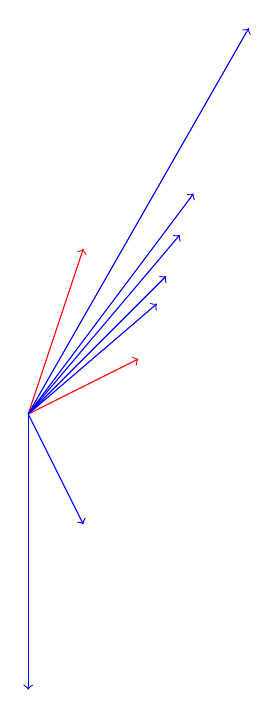
\begin{tikzpicture}[scale=.7]
	    % abscisa y ordenada
	    \tkzInit[xmax= 3,xmin=0,ymax=6,ymin=0]
	    \tiny\tkzLabelXY[opacity=0.6,step=1, orig=false]
	    % label x, f(x)
	    \tkzDrawX[opacity=0.6,label=x,right=0.3]
	    \tkzDrawY[opacity=0.6,label=f(x),below = -0.6]
	    \draw[red, ->](0,0)--(2,1);
	    \draw[red, ->](0,0)--(1,3);
	    \draw[blue, ->](0,0)--(7/3,2);
	    \draw[blue, ->](0,0)--(5/2,5/2);
	    \draw[blue, ->](0,0)--(11/4,13/4);
	    \draw[blue, ->](0,0)--(3,4);
	    \draw[blue, ->](0,0)--(4,7);
	    \draw[blue, ->](0,0)--(1,-2);
	    \draw[blue, ->](0,0)--(0,-5);
	\end{tikzpicture}
    \end{center}

%--------------------3.
\item resolver el ejercicio 2 si $C=tA+B$.\\\\
    Respuesta.-\; 
    \begin{center}
	\begin{tabular}{clcl}
	    Si&$t=\frac{1}{3}$&$\Longrightarrow$&$C=(\frac{5}{3},\frac{10}{3})$\\\\
	    Si & $t=\frac{1}{2}$ & $\Longrightarrow$ & $C=(2,\frac{7}{2})$ \\\\
	    Si & $t=1$ & $\Longrightarrow$ & $C=(\frac{5}{2},\frac{15}{4})$ \\\\
	    Si & $t=2$ & $\Longrightarrow$ & $C=(3,4)$ \\\\
	    Si & $t=-1$ & $\Longrightarrow$ & $C=(5,5)$ \\\\
	    Si & $t=-2$ & $\Longrightarrow$ & $C=(-1,2)$ \\\\
	    Si & $t=\frac{3}{4}$ & $\Longrightarrow$ & $C=(-3,1)$ \\\\
	\end{tabular}
    \end{center}
    \begin{center}
	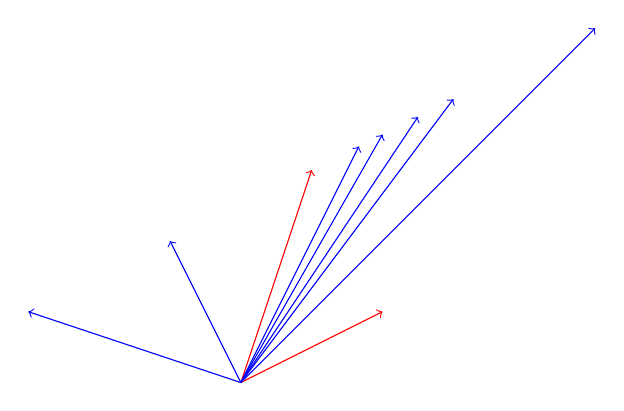
\begin{tikzpicture}[scale=.9]
	    % abscisa y ordenada
	    \tkzInit[xmax= 3,xmin=-3,ymax=3,ymin=0]
	    \tiny\tkzLabelXY[opacity=0.6,step=1, orig=false]
	    % label x, f(x)
	    \tkzDrawX[opacity=0.6,label=x,right=0.3]
	    \tkzDrawY[opacity=0.6,label=f(x),below = -0.6]
	    \draw[red, ->](0,0)--(2,1);
	    \draw[red, ->](0,0)--(1,3);
	    \draw[blue, ->](0,0)--(5/3,10/3);
	    \draw[blue, ->](0,0)--(2,7/2);
	    \draw[blue, ->](0,0)--(5/2,15/4);
	    \draw[blue, ->](0,0)--(3,4);
	    \draw[blue, ->](0,0)--(5,5);
	    \draw[blue, ->](0,0)--(-1,2);
	    \draw[blue, ->](0,0)--(-3,1);
	\end{tikzpicture}
    \end{center}

%--------------------4.
\item Sean $A=(2,1)$, $B=(1,3)$ y $C=xA+yB$, en donde $x$ e $y$ son escalares.
\begin{enumerate}[\bfseries a)]
    
    %----------a)
    \item Trazar el vector que une el origen a $C$ para cada uno de los siguientes pares de valores de $x$ e $y$: $x=y=\frac{1}{2}$; $x=\frac{1}{4},\;y = \frac{3}{4}$; $x=\frac{1}{3}, \; y=\frac{2}{3}$; $x=2,\; y=-1$; $x=3,\; y=-2$; $x=-\frac{1}{2},\; y=\frac{3}{2}$; $x=-1,\; y=2$.\\\\
	Respuesta.-\; 
	\begin{center}
	    \begin{tabular}{clcl}
		Si&$x=y=\frac{1}{2}$&$\Longrightarrow$&$C=\left(\frac{3}{2},2\right)$\\\\
		Si & $x=\frac{1}{4},\;y = \frac{3}{4}$ & $\Longrightarrow$ & $C=\left(\frac{5}{4},\frac{5}{2}\right)$ \\\\
		Si & $x=\frac{1}{3}, \; y=\frac{2}{3}$ & $\Longrightarrow$ & $C=\left(\frac{4}{3},\frac{7}{3}\right)$ \\\\
		Si & $x=2,\; y=-1$ & $\Longrightarrow$ & $C=(3,-1)$ \\\\
		Si & $x=3,\; y=-2$ & $\Longrightarrow$ & $C=(4,-3)$ \\\\
		Si & $x=-\frac{1}{2},\; y=\frac{3}{2}$ & $\Longrightarrow$ & $C=\left(\frac{1}{2},4\right)$ \\\\
		Si & $x=-1,\; y=2$ & $\Longrightarrow$ & $C=(0,5)$ \\\\
	    \end{tabular}
	\end{center}
	\begin{center}
	    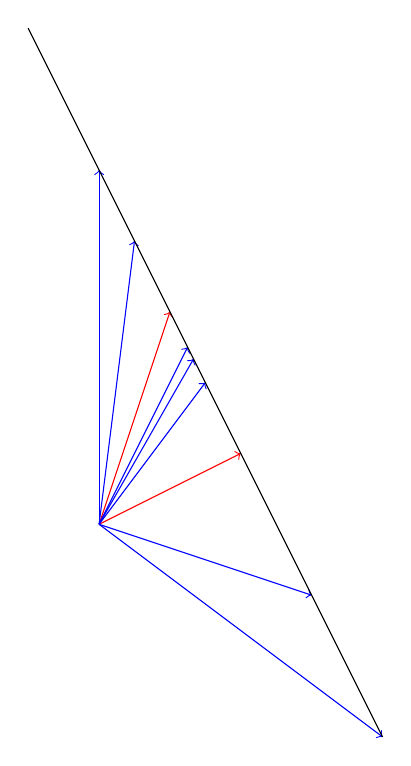
\begin{tikzpicture}[scale=.9]
		% abscisa y ordenada
		\tkzInit[xmax= 4,xmin=-3,ymax=4,ymin=-3]
		\tiny\tkzLabelXY[opacity=0.6,step=1, orig=false]
		% label x, f(x)
		\tkzDrawX[opacity=0.6,label=x,right=0.3]
		\tkzDrawY[opacity=0.6,label=f(x),below = -0.6]
		\draw[red, ->](0,0)--(2,1);
		\draw[red, ->](0,0)--(1,3);
		\draw[blue, ->](0,0)--(3/2,2);
		\draw[blue, ->](0,0)--(5/4,5/2);
		\draw[blue, ->](0,0)--(4/3,7/3);
		\draw[blue, ->](0,0)--(3,-1);
		\draw[blue, ->](0,0)--(4,-3);
		\draw[blue, ->](0,0)--(1/2,4);
		\draw[blue, ->](0,0)--(0,5);
		\draw[black](-1,7)--(4,-3);
	    \end{tikzpicture}
	\end{center}
    
    %----------b)
    \item ¿Qué conjunto es el de los puntos $C$ obtenidos cuando $x$ e $y$ toman todos los valores reales tales que $x+y=1$? (Hacer una conjetura y mostrar el lugar geométrico en la figura. No hacer la demostración).\\\\
	Respuesta.-\; Sea $x=3,\; y=-2$  y $x=-2,\; y=3$ podemos graficar el conjunto de los puntos $C$ tales que $x+y=1$.\\\\ 
    
    %----------c)
    \item Dar una idea del conjunto de todos los puntos $C$ obtenidos al variar independientemente $x$ e $y$ en los intervalos $0\leq x\leq 1, \; 0\leq y \leq 1,$ y hacer una representación de ese conjunto.\\\\
	Respuesta.-\; 
	\begin{center}
	    \begin{tikzpicture}[scale=.9]
		% abscisa y ordenada
		\tkzInit[xmax= 4,xmin=-3,ymax=4,ymin=-3]
		\tiny\tkzLabelXY[opacity=0.6,step=1, orig=false]
		% label x, f(x)
		\tkzDrawX[opacity=0.6,label=x,right=0.3]
		\tkzDrawY[opacity=0.6,label=f(x),below = -0.6]
		\draw[->](0,0)--(2,1);
		\draw[->](2,1)--(3,4);
		\draw[->](0,0)--(3,4);
	    \end{tikzpicture}
	\end{center}
    
    %----------d)
    \item ¿Qué conjunto es el de todos los puntos $C$ obtenidos si $x$ varía en el intervalo $0\leq x \leq 1$ e $y$ recorre todos los números reales?.\\\\
	Respuesta.-\; La banda horizontal obtenida sumando $xA$ a la línea $y = \frac{1}{3}x$ para cada uno $0 \leq x \leq 1$.\\\\

    %----------e)
    \item ¿Qué conjunto resulta si $x$ e $y$ recorren ambos todos los números reales?.\\\\
	Respuesta.-\; Todo $R^2$.\\\\

\end{enumerate}

%--------------------5.
\item Sean $A=(2,1)$ y $B=(1,3)$. Demostrar que todo vector $C=(c_1,c_2)$ de $V_2$ puede expresarse en la forma $C = xA+yB$. Expresar $x$ e $y$ en función de $c_1$ y $c_2$.\\\\
    Demostración.-\; Ya que $$C=xA+yB = (2x+y,x+3y)  = (c_1,c_2)$$
    se tiene $c_1 = 2x+y\;$ y $\;c_2 = x+3y$ de donde $$y=\dfrac{1}{5}(2c_2-c_1)$$  $$\;x=\dfrac{1}{5}(3c_1-c_2)$$
    Esto demuestra que cualquier vector en $\mathbb{R}^2$ se puede obtener como $xA+yB$ dado $C=(c_1,c_2)$ que calculamos.\\\\

%--------------------6.
\item Sea $A=(1,1,1)$, $B=(0,1,1)$ y $C=(1,1,0)$ tres vectores de $V_3$ y $D=xA+yB+zC$, donde $x$, $y$ $z$ son escalares.
\begin{enumerate}[\bfseries a)]

    %----------a)
    \item Determinar los componentes de $D$.\\\\
	Respuesta.-\; Tenemos que $D=x(1,1,1)+y(0,1,1)+z(1,1,0)$ de donde $D=(x,x,x)+(0,y,y)+(z,z,0)$
	así, $$D=(x+z,x+y+z,x+y)$$\\

    %----------b)
    \item Si $D=0$ demostrar que $x=y=z=0$.\\\\
	Demostración.-\; Sea $D=0=(0,0,0)$ entonces 
	\begin{center}
	    \begin{tabular}{rcl}
		$x+z=0$&$\Longrightarrow$&$x=-z$\\	
		$x+y+z=0$&$\Longrightarrow$&$y=0$\\
		$x+y=0$&$\Longrightarrow$&$x=-y$\\
	    \end{tabular}
	\end{center}
	de donde concluimos que $x=y=z=0$.\\\\

    %----------c)
    \item Hallar $x, y, z$ tales que $D=(1,2,3)$.\\\\
	Respuesta.-\; 
	\begin{center}
	    \begin{tabular}{rcll}
		$x+z=1$&$\Longrightarrow$&$z=1-x$&$\Longrightarrow z=-1$\\
		$x+y+z=2$&$\Longrightarrow$&$x+y+1-x=2$&$\Longrightarrow y=1$\\
		$x+y=3$&$\Longrightarrow$&$x+1=3$&$\Longrightarrow x=2$\\\\
	    \end{tabular}
	\end{center}

\end{enumerate}

%--------------------7.
\item Sean $A=(1,1,1)$, $B=(0,1,1)$ y $C=(2,1,1)$ tres vectores de $V_3$ y $D=xA+yB+zC$, en donde $x,y,z$ son escalares.
\begin{enumerate}[\bfseries a)]

    %----------a)
    \item Determinar los componentes de $D$.\\\\
	Respuesta.-\; Sea $D=x(1,1,1)+y(0,1,1)+z(2,1,1)$ entonces $D=(x+2z,x+y+z,x+y+z)$.\\\\


    %----------b)
    \item Hallar $x,y,z$ no todos nulos, tales que $D=0$.\\\\
	Respuesta.-\; Sea $x=2$, $y=-1$ y $z=-1$, entonces $$D=(x+2z,x+y+z,x+y+z)=(2-2,2-1-1,2-1-1)=(0,0,0)=O$$ \\

    %----------c)
    \item Demostrar que ninguna elección de $x,y,z$ hace $D=(1,2,3)$.\\\\
	Demostración.-\; Sea 
	\begin{center}
	    \begin{tabular}{rcll}
		$x+2z=1$&$\Longrightarrow$&$x=1-2z$&\\
		$x+y+z=2$&$\Longrightarrow$&$1-2z+y+z=2$&$\Longrightarrow y=z+1$\\
		$x+y+z=3$&$\Longrightarrow$&$1-2z+z+1+z=3$&$\Longrightarrow 2=3$\\
	    \end{tabular}
	\end{center}
	de donde encontramos un absurdo al declarar que $2=3$, por lo tanto no existe ninguna elección que satisfaga a $D=(1,2,3)$.\\\\

\end{enumerate}

%--------------------8.
\item Sean $A=(1,1,1,0)$, $B=(0,1,1,1)$, $C=(1,1,0,0)$ tres vectores de $V_4$ y $D=xA+yB+zC$ siendo $x,y,z$ escalares.
\begin{enumerate}[\bfseries a)]

    %----------a)
    \item Determinar los componentes de $D$.\\\\
	Respuesta.-\; Se tiene $D=x(1,1,1,0)+y(0,1,1,1)+z(1,1,0,0)$ entonces $D=(x+z,x+y+z,x+y,y)$\\\\

    %----------b)
    \item Si $D=0$, Demostrar que $x=y=z=0$\\\\
	Respuesta.-\; 
	\begin{center}
	\begin{tabular}{rcl}
	    $x+z=0$&&\\
	    $x+y+z=0$&$\Longrightarrow$&$z=0$\\
	    $x+y=0$&$\Longrightarrow$&$x=0$\\
	    $y=0$&&\\
	\end{tabular}
	\end{center}
	Por lo tanto $x=y=z=0$.\\\\

    %----------c)
    \item Hallar $x,y,z$ tales que $D=(1,5,3,4)$.\\\\
	Respuesta.-\;
	\begin{center}
	\begin{tabular}{rcl}
	 $x+z=1$&&\\
	 $x+y+z=5$&$\Longrightarrow$&$z=2$\\
	 $x+y=3$&$\Longrightarrow$&$x=-1$\\
	 $y=4$&&\\
	\end{tabular}
	\end{center}
	Por lo tanto $x=-1$, $y=4$ y $z=2$.\\\\

    %----------d)
    \item Demostrar que ninguna elección de $x,y,z$ hace $D=(1,2,3,4)$.\\\\
	Demostración.-\; La demostración es similar al problema 7c.\\\\

\end{enumerate}

%--------------------9.
\item En $V_n$ demostrar que dos vectores paralelos a un mismo vector son paralelos entre sí.\\\\
    Demostración.-\; Por definición de vectores paralelos se tiene $c_1A=C$ y $c_2B=C$ de donde $c_1A=c_2B$, en vista de que $c_1\cdot c_2 \neq 0$ entonces $B=c_1c_2^{-1} A$, por lo tanto concluimos que $A$ y $B$ son paralelos entre sí.\\\\ 

%--------------------10.
\item Dados cuatro vectores no nulos $A,B,C,D$ de $V_n$ tales que $C=A+B$ y $A$ paralelo a $D$. Demostrar que $C$ es paralelo a $D$ si y sólo si $B$ es paralelo a $D$.\\\\
    Demostración.\;  Sea $B=A-C$ de donde $B=cD-c_1D$ así, $B=(c-c_1)D$, (sabemos que $c-c_1\neq 0$, ya que $B$ es distinto de $0$).\\
    Por el contrario supongamos que $B$ es paralelo a $D$. Dado que ambos $A$ y $B$ son paralelos entre sí, esto por el problema anterior. Entonces, tenemos $A=xB$ siendo $x$ un escalar distinto de $0$. Esto implica $$C=C=xB+B \Longrightarrow C = (1-x)B.$$ Por lo tanto si $C$ es paralelo a $B$ y $B$ paralelo a $D$ entonces $C$ es paralelo a $D$.\\\\ 

%--------------------11.
\item 
\begin{enumerate}[\bfseries a)]
    
    %----------a)
    \item Demostrar, para los vectores $V_n$ las propiedades de la adición y de la multiplicación por escalares dadas en el teorema 12.1\\\\
	Demostración.-\; Sea $A,B \in V_n$ donde $A=(a_1,a_2,...,a_n)$ y $B=(b_1,b_2,...,b_n)$ entonces para la conmutatividad de adición tenemos $$A+B=(a_1,a_2,...,a_n)+(b_1,b_2,...,b_n) = (a_1+b_1,a_2+b_2,...,a_n+b_n) = (b_1+a_1,b_2+a_1,...,b_n+a_n) = B+A$$
	Para la asociatividad de adición se tiene,
	\begin{center}
	    \begin{tabular}{rcl}
		$A+(B+C)$&$=$&$(a_1,a_2,...,a_n)+\left[(b_1,b_2,...,b_n)+(c_1,c_2,...,c_n)\right]$\\
		&$=$&$\left[a_1+(b_1+c_1),a_2+(b_2+b_3),...,a_n+(b_n+c_n)\right]$\\
		&$=$&$\left[(a_1+b_1)+c_1,(a_2+b_2)+c_3,...,(a_n+b_n)+c_n\right]$\\
		&$=$&$(A+B)+C$\\
	    \end{tabular}
	\end{center}
	Luego para la asociatividad de la multiplicación escalar tenemos,
	\begin{center}
	    \begin{tabular}{rcl}
		$c(dA)$&$=$&$c\left[d(a_1,a_2,...,a_n)\right]$\\
		&$=$&$c(da_1,da_2,...,da_n)$\\
		&$=$&$\left[(cd)a_1,(cd)a_2,...,(cd)a_n\right]$\\
		&$=$&$(cd)(a_1,a_2,...,a_n)$\\
		&$=$&$(cd)A$\\
	    \end{tabular}
	\end{center}
	Para la primera ley distributiva se tiene,
	\begin{center}
	    \begin{tabular}{rcl}
		$c(A+B)$&$=$&$c\left[(a_1,a_2,...,a_n)+(b_1,b_2,...,b_n)\right]$\\
		&$=$&$\left[c(a_1+b_1),c(a_2+b_2),...,c(a_n+b_n)\right]$\\
		&$=$&$(ca_1+c_b1,ca_2+cb_2,...,ca_n+cb_n)$\\
		&$=$&$(c_1,ca_2,...,ca_n)+(cb_1,cb_2,...,cb_n)$\\
		&$=$&$c(a_1,a_2,...,a_n)+c(b_1,b_2,...,b_n)$\\
		&$=$&$cA+cB$\\
	    \end{tabular}
	\end{center}
	Para la segunda ley distributiva obtenemos,
	\begin{center}
	    \begin{tabular}{rcl}
		$(c+d)A$&$=$&$(c+d)(a_1,a_2,...,a_n)$\\
		&$=$&$(ca_1+cb_1,ca_2+cb_2,...,ca_n+da_n)$\\
		&$=$&$(c_1,ca_2,...,ca_n)+(cb_1,cb_2,...,cb_n)$\\
		&$=$&$c(a_1,a_2,...,a_n)+d(a_1,a_2,...,a_n)$\\
		&$=$&$cA+dA$\\\\
	    \end{tabular}
	\end{center}

    %----------b)
    \item Mediante vectores geométricos en el plano, representar el significado geométrico de las dos leyes distributivas $(c+d)A=cA+dA$ y $c(A+B) = cA+cB$.\\\\
	Respuesta.-\; La ley distributiva $(c + d) A = cA + dA$ significa que el vector $(c + d)$ Ase obtiene sumando la flecha $dA$ al final de la flecha $cA$.\\
La ley distributiva $c (A + B) = cA + cB$ significa que el vector $c (A + B)$ es el vértice del paralelogramo formado por $cA$ y $cB$.\\\\

\end{enumerate}

%--------------------12.
\item Si un cuadrilátero $OABC$ de $V_2$ es un paralelogramo que tiene $A$ y $C$ como vértices opuestos, demostrar que $A+\frac{1}{2}(C-A) =\frac{1}{2}B$. ¿Qué teorema relativo a los paralelogramos puede deducirse de esta igualdad?.\\\\
    Demostración.-\; Dado que este es un paralelogramo, tenemos $B=A+C$. Y por tanto,
    $$B=A+C\; \Longrightarrow\; \dfrac{1}{2}B=\dfrac{1}{2}(A+C)\; \Longrightarrow\; \dfrac{1}{2}B = A + \dfrac{1}{2}C - \dfrac{1}{2} A \;\Longrightarrow \; \dfrac{1}{2}B = A + \dfrac{1}{2}(C-A)$$\\

\end{enumerate}


\section{Producto escalar}

%--------------------definición 12.3
\begin{tcolorbox}[colframe=white]
    \begin{def.}[Producto escalar ó interior de dos vectores] Si $A=(a_1,a_2,...,a_n)$ y $B=(b_1,b_2,...,b_n)$ son dos vectores de $V_n$ su producto escalar se representa con $A\cdot B$ y se define con la igualdad $$A\cdot B = \sum_{k=1}^n a_k\cdot b_k$$
    \end{def.}
\end{tcolorbox}

%--------------------teorema 12.2
\begin{teo} Para todos los vectores $A,B,C$ de $V_n$ y todos los escalares $c$ se tienen las propiedades siguientes:
\begin{center}
\begin{tabular}{cll}
    
    %----------(a)
     \textbf{(a)}&$A\cdot B = B\cdot A$& (ley conmutativa).\\

    %----------(b)
    \textbf{(b)} & $A\cdot(B+C) = A\cdot B + A\cdot C$ & (ley distributiva) \\

    %----------(c)
    \textbf{(c)} & $c(A\cdot B) = (cA)\cdot B = A\cdot (cB)$ & (homogeneidad) \\

    %----------(d)
    \textbf{(d)} & $A\cdot A > 0$ si $A\neq O$ & (positivadad) \\

    %----------(e)
    \textbf{(e)} & $A\cdot A = 0$ si $A=O$ & \\\\

\end{tabular}    
\end{center}
    Demostración.-\; Comencemos demostrando el inciso $(a)$ que es un consecuencia de la definición. $$A\cdot B = \sum_{k=1}^n a_kb_k = (a_1\cdot b_1) + (a_2\cdot b_2) + ... + (a_n\cdot b_n) = (b_n+a_n)+(b_2+a_n)+...+(b_n+a_n) = \sum_{k=1}^n b_k a_k = B\cdot A$$ 
    Las demostraciones $(b)$ y $(c)$ se demuestran con la definición de producto escalar, la definición de vectores y el teorema 12.1.\\
    Para demostrar las dos últimas, usamos la relación $A\cdot A = \sum a_k^2$. Puesto que cada térmi es no negativo, la suma es es no negativa. Además, la suma es cero si y sólo si cada término de la suma es cero y esto tan sólo puede ocurrir si $A=O$.\\\\

\end{teo}

%--------------------teorema 12.3
\begin{teo}[Desigualdad de Cauchy-Schwarz] Si $A$ y $B$ son vectores de $V_n$, tenemos $$(A\cdot B)^2 \leq (A\cdot A)(B\cdot B) \qquad \mbox{12.2}$$.
Además, el signo de desigualdad es el válido si y sólo si uno de los vectores es el producto de otro por un escalar.\\\\
    Demostración.-\; Expresando cada uno de los miembros de (12.2) en función de los componentes, obtenemos $$\left(\sum_{k=1}^n a_kb_k\right)^2\leq \left(\sum_{k=1}^n a_k^2\right)\left(\sum_{k=1}^n b_k^2\right)$$
    que es la desigualdad ya demostrada en el teorema I.41.\\\\
    Presentaremos otra demostración de 12.2 que no utiliza los componentes.\\
    Tal demostración es interesante porque hace ver que la desigualdad de Cauchy-Schwarz es una consecuencia de las cinco propiedades del producto escalar que se citan en el teorema 12.2 y no depende de la definicón que se utilizó para deducir esas propiedades.\\
    Para llevar a acabo esta demostración, observemos primero que 12.2 es trivial si $A$ ó $B$ es el vector cero. Por tanto, podemos suponer que $A$ y $B$ son ambos no nulos. Sea $C$ el vector 
    $$C=xA-yB, \quad \mbox{donde}\; x=B\cdot B \quad \mbox{y} \quad y=A\cdot B$$
    Las propiedades d) y e) implican que $C\cdot C \geq 0$. Cuando expresamos esto en función de $x$ e $y$, resulta 12.2. Para expresar $C\cdot C$ en función de $x$ e $y$, utilizamos las propiedades a), b) y c) obteniendo $$C\cdot C = (xA-yB)\cdot (xA-yB) = x^2(A\cdot A) - 2xy(A\cdot B) + y^2(B\cdot B).$$
    Utilizando las definiciones de $x$ e $y$ como también la desigualdad $C\cdot C\leq 0$, se llega a $$(B\cdot B)^2\cdot(A\cdot A) -2(A\cdot B)^2(B\cdot B)+(A\cdot B)^2(B\cdot B)\geq 0$$
    La propiedad d) implica que $B\cdot B \geq 0$ puesto que $B\neq 0$, con lo que podemos dividir por $(B\cdot B)$ obteniendo $$(B\cdot B)(A\cdot A)-(A\cdot B)^2\geq 0$$
    que coincide con 12.2. Esto también demuestra que el signo igual es válido en 12.2 si y sólo si $C=0$. Pero $C=0$ si y sólo si $xA=yB$. A su vez, esta igualdad se verifica si y sólo si uno de los vectores es el producto del otro por un escalar.\\\\

\end{teo}


\section{Longitud o norma de un vector}

%--------------------definicion 12.4
\begin{tcolorbox}[colframe=white]
    \begin{def.} si $A$ es un vector en $V_n$ su longitud o norma se designa con $\|A\|$ y se define mediante la igualdad $$\|A\| = (A\cdot A)^{1/2}$$
    \end{def.}
\end{tcolorbox}

\begin{teo} Si $A$ es un vector de $V_n$ y $c$ un escalar, tenemos las siguientes propiedades.
\begin{center}
    \begin{tabular}{rcl}
	\textbf{a)}&$\|A\|>0$ si $A\neq 0$&(Positividad)\\	
	\textbf{b)}&$\|A\|=0$ si $A=0$&\\	
	\textbf{c)}&$\|cA\|=\left|c\right|\|A\|$&(homogeneidad)\\
    \end{tabular}
\end{center}

    Demostración.-\; Las propiedades a) y b) son consecuencia inmediata de las propiedades d) y e) del teorema 12.2. Para demostrar c) utilizamos la propiedad de homogeneidad del producto escalar obteniendo $$\|cA\|=(cA\cdot cA)^{1/2} = (c^2A\cdot A)^{1/2} ) (c^2)^{1/2}(A\cdot A)^{1/2} = |c|\|A\|.$$
    La desigualdad de Cauchy-Schwarz también se puede expresar en función de la norma. Ella establece que $$(A\cdot B)^2 \leq \|A\|^2 \|B\|^2\qquad \mbox{12.3}$$ $$o$$ $$|A\cdot B| = \|A\|\|B\| \qquad \mbox{12.4}$$\\\\

\end{teo}

%--------------------teorema 12.5
\begin{teo}[Desigualdad triangular]. Si $A$ y $B$ son vectores de $V_n$, tenemos $$\|A+B\| \leq \|A\|+\|B\|.$$\\
    Demostración.-\; para evitar las raíces cuadradas, escribimos la desigualdad triangular en la forma equivalente $$\|A\cdot B\|^2 = \left(\|A\|+\|B\|\right)^2\qquad \mbox{12.5}$$
    El primer miembro de 12.5 es $$\|A+B\|^2 = (A+B)\cdot (A+B) = A\cdot A + 2A\cdot B + B\cdot B = \|A\|^2 + 2A\cdot B + B\cdot B = \|A\|^2 + 2A\cdot B + \|B\|^2$$
    mientras que el segundo miembro es $$\left(\|A\|+\|B\|\right)^2 = \|A\|^2 + 2\|A\|\|B\|+\|B\|^2$$
    Comparando esas dos fórmulas, vemos que 12.5 es válida si y sólo si se tiene $$A\cdot B \leq \|A\|\|B\|\qquad 12.6$$
    Pero $A\cdot B\leq A\cdot B$ con lo que 12.6 resulta de la desigualdad de Cauchy-Schwarz, en la forma 12.4. Esto prueba que la desigualdad triangular es consecuencia de la desigualdad de Cauchy-Schwarz.\\
    La proposición reciproca también es cierta. Esto es, si la desigualdad triangular es cierta también lo es 12.6 para $A$ y para $-A$, de lo que obtenemos 12.3. Así pues, la desigualdad triangular y la de Cauchy-Schwarz son lógicamente equivalentes. Además, el signo de igualdad vale en una si y sólo si vale en la otra. Con lo que se complementa la demostración del teorema 12.5.\\\\

\end{teo}

\section{Ortogonalidad de vectores}

%--------------------definicion 12.5
\begin{tcolorbox}[colframe=white]
\begin{def.} Dos vectores $A$ y $B$ de $V_n$ son perpendiculares u ortogonales si $A\cdot B=0$.
\end{def.}
\end{tcolorbox}


\section{Ejercicios}

\begin{enumerate}[\Large\bfseries 1.]

%--------------------1.
\item Sean $A=(1,2,3,4)$, $B=(-1,2,-3,0)$ y $C=(0,1,0,1)$ tres vectores de $V_4$. Calcular cada uno de los siguientes productos.
\begin{enumerate}[\bfseries (a)]

    %----------(a)
    \item $A\cdot B = \sum\limits_{k=1}^4 a_kb_k = 1\cdot (-1) + 2\cdot 2 + 3\cdot (-3) + 4\cdot 0 = -1 + 4 - 9 + 0 = -6$.\\\\ 

    %----------(b)
    \item $B\cdot C = (-1)\cdot 0 + 2\cdot 1 + (-3)\cdot 0 + 0\cdot 1 = 2$.\\\\

    %----------(c)
    \item $A\cdot C = 1\cdot 0 + 2\cdot 1 + 3\cdot 0 + 4\cdot 1 = 6$.\\\\

    %----------(d)
    \item $A\cdot(B+C) = A\cdot B + A\cdot C = (-6) + 6 = 0$.\\\\

    %----------(e)
    \item $(A-B)\cdot C = A\cdot C - B \cdot C = 6 - 2 = 4$.\\\\

\end{enumerate}

%--------------------2.
\item Dados tres vectores $A=(2,4,-7)$, $B=(2,6,3)$ y $C=(3,4,-5)$. En cada una de las expresiones siguientes se pueden introducir paréntesis de una sola manera para obtener una expresión que tenga sentido. Introducir paréntesis y efectuar las operaciones.
\begin{enumerate}[\bfseries ]
    
    %----------(a)
    \item $(A\cdot B)C = \left[2\cdot 2 + 4\cdot 6 + (-7)\cdot 3\right]C = 7(3,4,-5) = (21,28,-35)$.\\\\

    %----------(b)
    \item $A\cdot (B + C) = (2,4,-7)\cdot (5,10,-2) = 2\cdot 5 + 4\cdot 10 + (-7)\cdot(-2) = 64$.\\\\ 

    %----------(c)
    \item $(A+B)\cdot C = (4,10,-4)\cdot (3,4,-5) = 4\cdot 3 + 10 \cdot 4, (-4)\cdot (-5) = 72$.\\\\

    %----------(d)
    \item $A(B\cdot C) = A\left[2\cdot 3 + 6\cdot 4 + 3\cdot (-5)\right] = (2,4,-7)15 = (30,60,-105)$.\\\\

    %----------(e)
    \item $A/(B\cdot C) = A/\left[2\cdot 3 + 6\cdot 4 + 3\cdot (-5)\right] = (2,4,-7)/15 = \left(\dfrac{2}{15},\dfrac{4}{15},-\dfrac{7}{15}\right)$.\\\\

\end{enumerate}

%-------------------3.
\item Demostrar si es o no cierta la proposición siguiente referentes a vectores en $V_n$: Si $A\cdot B=A\cdot C$ y $A\neq 0$, es $B=C$.\\\\
    Demostración.-\; Esta proposición es falsa ya que si $A=(1,1,1)$, $B=(1,-1,0)$ y $C=(0,-1,1)$ entonces $$A\cdot B = 1\cdot 1 + 1\cdot(-1)+1\cdot 0 = 0, \qquad A\cdot C = 1\cdot 0 + 1\cdot(-1)+1\cdot 1 = 0$$
    de donde $B\neq C$.\\\\ 

%--------------------4.
\item 

\end{enumerate}
